\subsection{Physical Application: The Tautochrone Problem}
    
    We wish to find a curve such that, if an object starts on any point along this curve, the time that it requires to slide down to the origin is constant, moving without friction only by the force of gravity. It is important to remark that this problem does not necessarily require fractional derivatives, although the problem (proposed by Abel about three centuries ago \cite{kisela2008fractional}) was one of the first applications of fractional calculus.
    
    \begin{figure}[H]
        \centering
        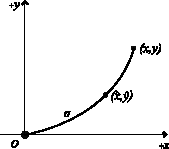
\includegraphics[scale=1.75]{files/taut.pdf}
        \caption{Tautochrone problem.}
        \label{fig:taut}
    \end{figure}
    
    Suppose we start somewhere in the $xy$ plane in a point $(x,y)$. Let $\sigma$ be the distance along the \textbf{curve} from the origin. Let us analyze the energy in a point $(\hat{x},\hat{y})$. 
    
    The energy conservation law states that $E_0 = E_f$, hence 
    
    \begin{equation}
        mgy = \dfrac{1}{2}mv^2 + mg\hat{y}
    \end{equation}
    
    Taking $v=\dfrac{d\sigma}{dt}$, we have
    \begin{align*}
        mgy &= \dfrac{1}{2}m\left(\dfrac{d\sigma}{dt}\right)^2 + mg\hat{y}\\
        \left(\dfrac{d\sigma}{dt}\right)^2 &= 2g(y-\hat{y})
    \end{align*}
    
    Note that $d\sigma/dt < 0$, since the object is approaching the origin. On the other hand, we assume $\sigma=\sigma(\hat{y}(t))$, therefore
    \begin{equation*}
        \dfrac{d\sigma}{dt}=\dfrac{d\sigma}{d\hat{y}}\cdot\dfrac{d\hat{y}}{dt}=\sigma'\dfrac{d\hat{y}}{dt}
    \end{equation*}
    
    Applying this, we have
    
    \begin{align*}
        \sigma'\dfrac{d\hat{y}}{dt} &= -\sqrt{2g(y-\hat{y})}\\
        \sigma'\dfrac{d\hat{y}}{\sqrt{y-\hat{y}}}&=\sqrt{2g}dt
    \end{align*}
    
    Integrating from $\hat{y}=0$ to $\hat{y}=y$ and $t$ from $t=0$ to $t=T$
    
    \begin{align*}
        \int_0^y \sigma'\dfrac{d\hat{y}}{\sqrt{y-\hat{y}}} &= \sqrt{2g}\int_0^Tdt\\
        \Gamma\left(1-\frac{1}{2}\right)\left[
        \dfrac{1}{\Gamma\left(1-\frac{1}{2}\right)}\int_0^y\sigma'\dfrac{d\hat{y}}{(y-\hat{y})^{1-1+\frac{1}{2}}}\right] &= \sqrt{2g}T
    \end{align*}
    Clearly, the inside of the left side of the equation is a Caputo-type fractional derivative. Hence,
    \begin{equation}
        \mathcal { D } _ { c } ^ { \frac { 1 } { 2 } } \sigma ( y ) = \frac { \sqrt { 2 g } } { \Gamma \left( \frac { 1 } { 2 } \right) } T
    \end{equation}
    
    This is a fractional differential equation for the function $\sigma(y)$, with initial condition $\sigma(0)=0$ since arc length at the origin is 0.
    Applying theorem \ref{theo:rightinverse}, we can apply the $\frac{1}{2}$-integral and obtain the solution. 
    \begin{align*}
        J^{\frac{1}{2}} \left[\mathcal { D } _ { c } ^ { \frac { 1 } { 2 } } \sigma ( y )\right] &= J^{\frac{1}{2}} \left[\frac { \sqrt { 2 g } } { \Gamma \left( \frac { 1 } { 2 } \right) } T \right] \\
        &= \dfrac{1}{\Gamma\left(\frac{1}{2}\right)}\int_0^y \dfrac{\frac { \sqrt { 2 g } } { \Gamma \left( \frac { 1 } { 2 } \right) } T}{(y-\lambda)^{1-\frac{1}{2}}}d\lambda\\
        &= \dfrac{\sqrt{2g}}{\left[\Gamma\left(\frac{1}{2}\right)\right]^2}T\int_0^y\dfrac{d\lambda}{(y-\lambda)^{\frac{1}{2}}}
    \end{align*}
    Let $u=y-\lambda\rightarrow du = -d\lambda$, then
    \begin{align*}
        J^{\frac{1}{2}} \left[\mathcal { D } _ { c } ^ { \frac { 1 } { 2 } } \sigma ( y )\right] &= \dfrac{\sqrt{2g}T}{\left[\Gamma\left(\frac{1}{2}\right)\right]^2}\int_0^y \dfrac{du}{u^{\frac{1}{2}}}\\
        &= \dfrac{2\sqrt{2g}T}{\left[\Gamma\left(\frac{1}{2}\right)\right]^2}u^{\frac{1}{2}}\bigg\rvert_0^y\\
        \sigma(y)&= \dfrac{2\sqrt{2g}T}{\pi}y^{\frac{1}{2}}
    \end{align*}
    Recall the formula for the distance along a curve
    \begin{equation}
        \dfrac{d\sigma}{dy}=\sqrt{1+\left(\dfrac{dx}{dy}\right)^2}
    \end{equation}
    
    Replacing, we have 
    
    \begin{equation}
        \dfrac{dx}{dy }=\sqrt{\dfrac{2gT^2}{\pi^2y}-1}
    \end{equation}\label{eq:tautfin}
    
    The solution to the ordinary differential equation is the solution to the Tautochrone problem. We will not prove the analytic solution. The solution to equation \ref{eq:tautfin} is given by the parametric expression
    \begin{align}
        x = \dfrac{gT^2}{\pi^2}[t+\sin(t)]\\
        y = \dfrac{gT^2}{\pi^2}[1-\cos(t)]
    \end{align}
    We could take $T=\dfrac{\pi}{\sqrt{2g}}$ in order to obtain $A=1$ and draw the Tautochrone easily:
    
    \begin{figure}[H]
        \centering
        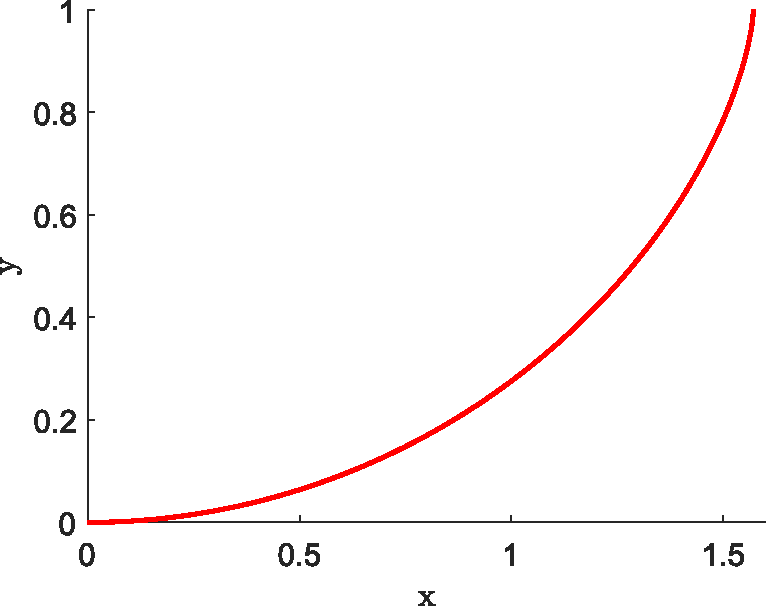
\includegraphics[scale=0.5]{files/tautochrone.pdf}
        \caption{Example of Tautochrone.}
    \end{figure}
    
    Which is an example of a Tautochrone: it does not matter the initial point along that curve, an object will always fall in the same time into the origin. It is important to mention that the tautochrone problem has a wide variety of procedures to be solved, but it is a clear example of fractional models in the real world.
